\documentclass[11pt]{article}
    % General document formatting
    \usepackage[margin=0.7in]{geometry}
    \usepackage[parfill]{parskip}
    \usepackage[utf8]{inputenc}
    \usepackage{graphicx}
    \usepackage{float}
    \usepackage{listings}
    \lstset{
  		basicstyle=\ttfamily,
  		columns=fullflexible,
  		frame=single,
  		breaklines=true,
	}
    
    % Related to math
    \usepackage{amsmath,amssymb,amsfonts,amsthm}
    
    % Document configuration
    \linespread{1.3}

\begin{document}

Hoffmann \& Sorn, 19.04.2019, Blockseminar Qualitätssicherung: Circle CI

\section {Was ist Circle CI?}

Circle CI ist eine Plattform für kontinuierliche Integration, die sowohl als Software as a Service als auch zur Installation auf eigener Hardware angeboten wird. Circle CI unterstützt dabei eine große Auswahl an gängigen Sprachen und Umgebungen mit ausführlich dokumentierten Beispielprojekten, an denen sich der Einsatz des Tools auch für CI-Anfänger einfach erlernen lässt.

\subsection {Was ist Kontinuierliche Integration?}

Die Idee hinter Kontinuierliche Integration ist, die einzelnen Komponenten einer Software während derer Entwicklung immer wieder zu einer Einheit zusammenzufügen. Üblicherweise beinhaltet dieser Vorgang nicht nur das Bauen des gesamten Codes, sondern auch das Ausführen von Tests, die sicherstellen sollen, dass sich durch die neu hinzugekommenen Änderungen keine Fehler in den Code eingeschlichen haben. Das Ziel dieses kontinuierlichen Bauens und Testens ist, die Qualität der entwickelten Software zu erhöhen, indem man Fehler frühzeitig bemerkt und verbessert.

Um ein eigenes Projekt kontinuierlich integrieren zu können, müssen ein paar Grundvoraussetzungen erfüllt sein. Der erste wichtige Schritt ist eine gemeinsame Codebasis, an der ein oder mehrere Entwickler arbeiten können. Eine Möglichkeit dafür sind Versionsverwaltung wie GIT oder SVN, in die alle Entwickler ihre Änderungen am Code einpflegen können. Eine weitere Voraussetzung ist die Möglichkeit, den Code automatisch bauen zu lassen. Für die meisten Sprachen gibt es hierfür Build-Tools, in denen die einzelnen Schritte des Übersetzen beschrieben werden können, um diese später automatisiert auszuführen. Beispiele wären hierfür Make oder CMake für C und C++ Projekte oder Maven für Java Projekte. Diese übernehmen nicht nur das übersetzen des eigenen Codes, sondern auch das Anbinden bereits bestehender Projekte, die als Abhängigkeiten definiert werden. Ziel hierbei ist es am Ende, die gesamte Software im besten Fall durch einen Befehl bauen zu können, ohne dass weitere Schritte von Hand notwendig sind. Eine weitere wichtige Voraussetzung ist es, Tests zu schreiben, mit denen sichergestellt werden kann, dass die Änderungen richtig funktionieren und nicht in bestehendem Code zu Fehlern führt. Hier können Tools wie SonarQube verwendet werden, die automatisch prüfen, welcher Anteil des Codes durch Tests bereits abgedeckt sind. Eine Erweiterung dieses Konzeptes wäre die Kontinuierliche Auslieferung. Diese beschreibt die automatisierte Auslieferung der Software, wenn diese erfolgreich integriert wurde. So könnte beispielsweise eine Webanwendung immer aktualisiert werden, sobald neue Features fertig entwickelt und getestet sind.

Auch wenn Kontinuierliche Integration gerade am Anfang mit zusätzlichem Aufwand verbunden ist, gibt es auf lange Sicht doch viele Vorteile, die den Einsatz in den meisten etwas umfangreicheren Softwareprojekten sinnvoll machen. Tauchen bei der Entwicklung Fehler auf, so können diese schnell und zeitnah behoben werden. Zudem ermöglicht es kontinuierliche Integration, immer eine sehr aktuelle Version der Software für Demonstrationen für beispielsweise Vertriebszwecke zur Verfügung zu haben. Eine Gefahr bei zu sehr langen Integrationszyklen ist es, dass die gemeinsame Codebasis sich zu stark in der Zeit ändert, in der ein neues, großes Feature entwickelt wird. Dies führt dazu, dass das einbinden des neuen Features zu einer langwierigen und komplizierten Aufgabe wird. Werden die Integrationszyklen hingegen klein gehalten, so wird der Gesamtaufwand einer Integration deutlich verringert.

\section{Einführung in die Verwendung von Circle CI}
Eine wichtige Frage bei der Einführung neuer Tools in ein Projekt ist immer, welche Vorteile und Nachteile sich aus der Verwendung ergeben. Bei Circle CI sehen wir uns dabei verstärkt die SaaS Variante an, da diese uns gerade am Anfang administrativen Aufwand und die Notwendigkeit von extra Hardware für die Installation erspart. Für die Integration des eigenen Projekts in Circle CI macht es im Grunde genommen keinen Unterschied, ob Code für das Projekt bereits geschrieben wurde, oder ob man mit einem neuen Projekt beginnt, in dem es weder Code noch Tests gibt. Im Code selbst sind keine Änderungen notwendig. Das Projekt benötigt lediglich eine Datei mit dem Namen \textit{config.yml} in einem Ordner \textit{.circleci}, den man in das Root Verzeichnis des Projektes ablegt, das in Circle CI gebaut werden soll.

\begin{figure}[H]
	\centering
  	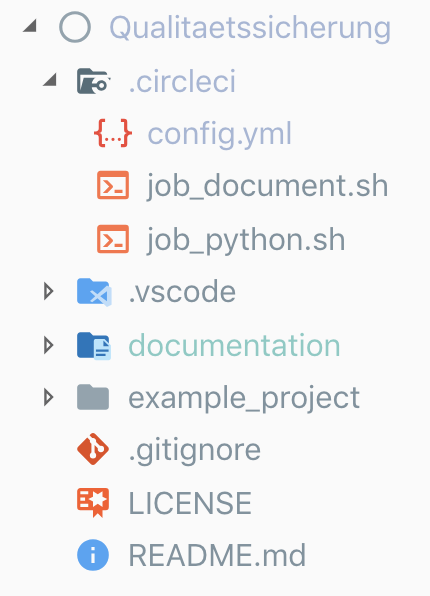
\includegraphics[width=0.3\linewidth]{../Images/Projektstruktur}
  	\caption{Projektstruktur mit Circle CI Konfigurationsdatei}
  	\label{fig:project-structure}
\end{figure}

Für Circle CI stellt diese Datei eine Anleitung mit einzelnen Arbeitsschritten bereit. Diese Datei in Verbindung mit der Autorisierung des Repositories genügen, um das Projekt von Circle CI bauen und testen zu können. Auf die genaue Konfiguration, die in der YAML Datei hinterlegt wird, gehen wir später etwas genauer anhand eines praktische Beispiels ein.

Ein weiteres Konzept von Circle CI zu Vereinfachung der Konfiguration sind sogenannte \textit{Orbs}, die es erlauben, bestimmte Konfigurationen als Pakete einfach wiederzuverwenden. Möchte man diese verwenden, so kann man die passenden in die eigene Konfiguration einbinden.

Über die Weboberfläche von Circle CI kann dann ausgewählt werden, welche der eigenen Projekte kontinuierlich gebaut werden sollen. Wird CircleCI beispielsweise in Verbindung mit GitHub betrieben, indem sich der Nutzer über seine GitHub Credentials authentifiziert, werden alle verfügbaren Projekte bereits in Dieser aufgelistet. Die Projekte, die gebaut werden sollen, müssen dann nur noch ausgewählt werden. Der Aufwand, eigene Projekte mit Circle CI kontinuierlich zu integrieren, ist damit minimal.

\begin{figure}[H]
	\centering
  	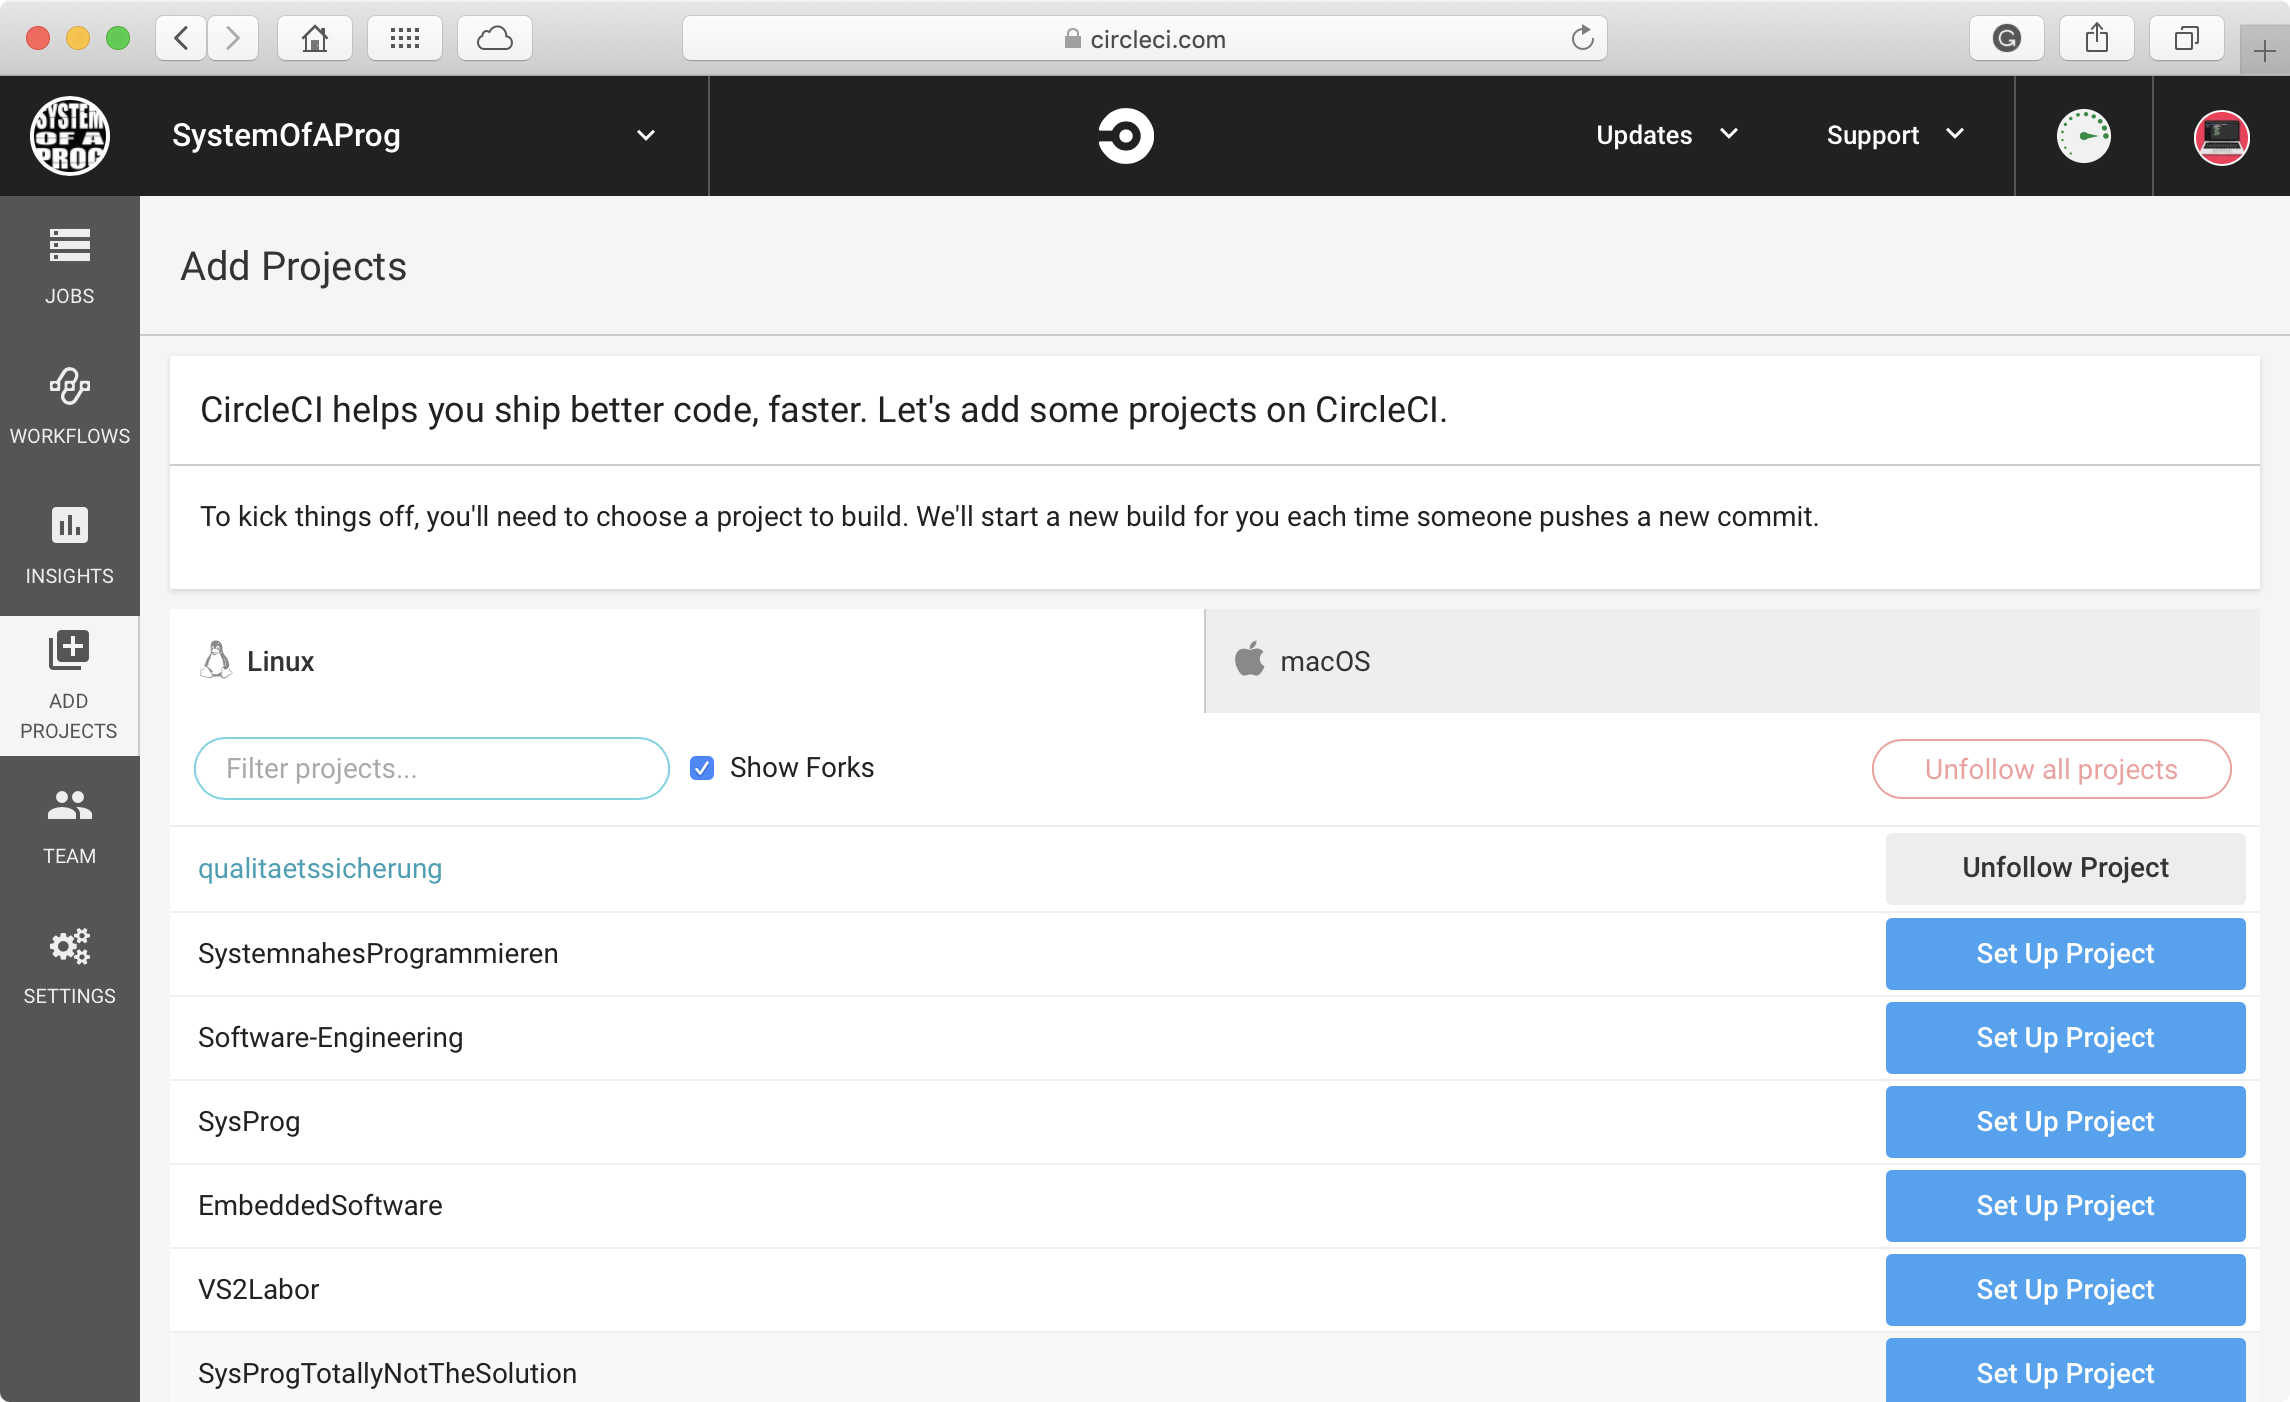
\includegraphics[width=1\linewidth]{../Images/Projekt_aktivieren}
  	\caption{Aktivierung eines Projektes in der Weboberfläche}
  	\label{fig:aktivieren}
\end{figure}

\subsection{Funktionsweise von Circle CI}
Circle CI testet Projekte in jeweils eigenen Containern oder Virtuellen Maschinen, die auf die Bedürfnisse der Projekte angepasst sind. Neben Linux basierten Containern und VMs können allerdings auch macOS basierte "Single Use" VMs für das Testen von iOS und macOS Anwendungen verwendet werden. Damit stellt Circle CI sicher, dass mehrere Jobs sehr einfach parallel laufen können, ohne dass sich diese gegenseitig beeinflussen. So wird sichergestellt, dass jeder Build in der selben, sauberen Umgebung ausgeführt wird.

\section{Fehlersuche, Debugging und Verbesserung der Performance}
\subsection{Test Metadaten}
CircleCI kann so konfiguriert werden, dass Testdaten und -ergebnisse gespeichert und eingesehen werden können. Dadurch können Informationen über die Performance der Tests erhalten und im Fall von auftretenden Fehlern und  gescheiterten Tests die Fehlerquellen schneller entdeckt werden. Über einen Konfigurationsschritt in der  YAML Datei kann das Sammeln von Testdaten aktiviert werden. Die Metadaten werden in einer XML Datei gespeichert  und können in der Insights Ansicht der Weboberfläche angezeigt werden. Außerdem besteht die Möglichkeit die Datei am Ende eines Jobdurchlaufes als Artefakt zur Verfügung gestellt werden.

\subsection{Debugging mit SSH}
CircleCI bietet im Fall eines auftretenden Fehlers die Möglichkeit zum Debuggen mit SSH. Dadurch ist es  möglich einzelne Jobs und Container zu erreichen und Log Files, laufende Prozesse und Directory Pfade zu  untersuchen. Um so eine Untersuchung zu starten, muss der verwendete GitHub Account einen SSH Key enthalten. Wenn das der Fall ist, kann in der Detailansicht eines abgeschlossenen Jobs über ein Dropdown Menü die Funktion "Rerun job with SSH" ausgeführt werden. Dadurch wird der Job erneut gestartet und kann nach der Eingabe des  SSH Keys durch die SSH Verbindung überwacht und untersucht werden. Für den Fall, dass beim Verbindungsversuch "Permission denied" Fehler auftreten, besteht die Möglichkeit über einzelne Kommandos die angegebenen Nutzer und Keys zu überprüfen.

\begin{figure}[H]
	\centering
  	
\includegraphics[width=0.25\linewidth]{../Images/SSH_Button}
  	\caption{Starten eines Jobs mit SSH Support}
  	\label{fig:ssh-button}
\end{figure}

\begin{figure}[H]
	\centering
  	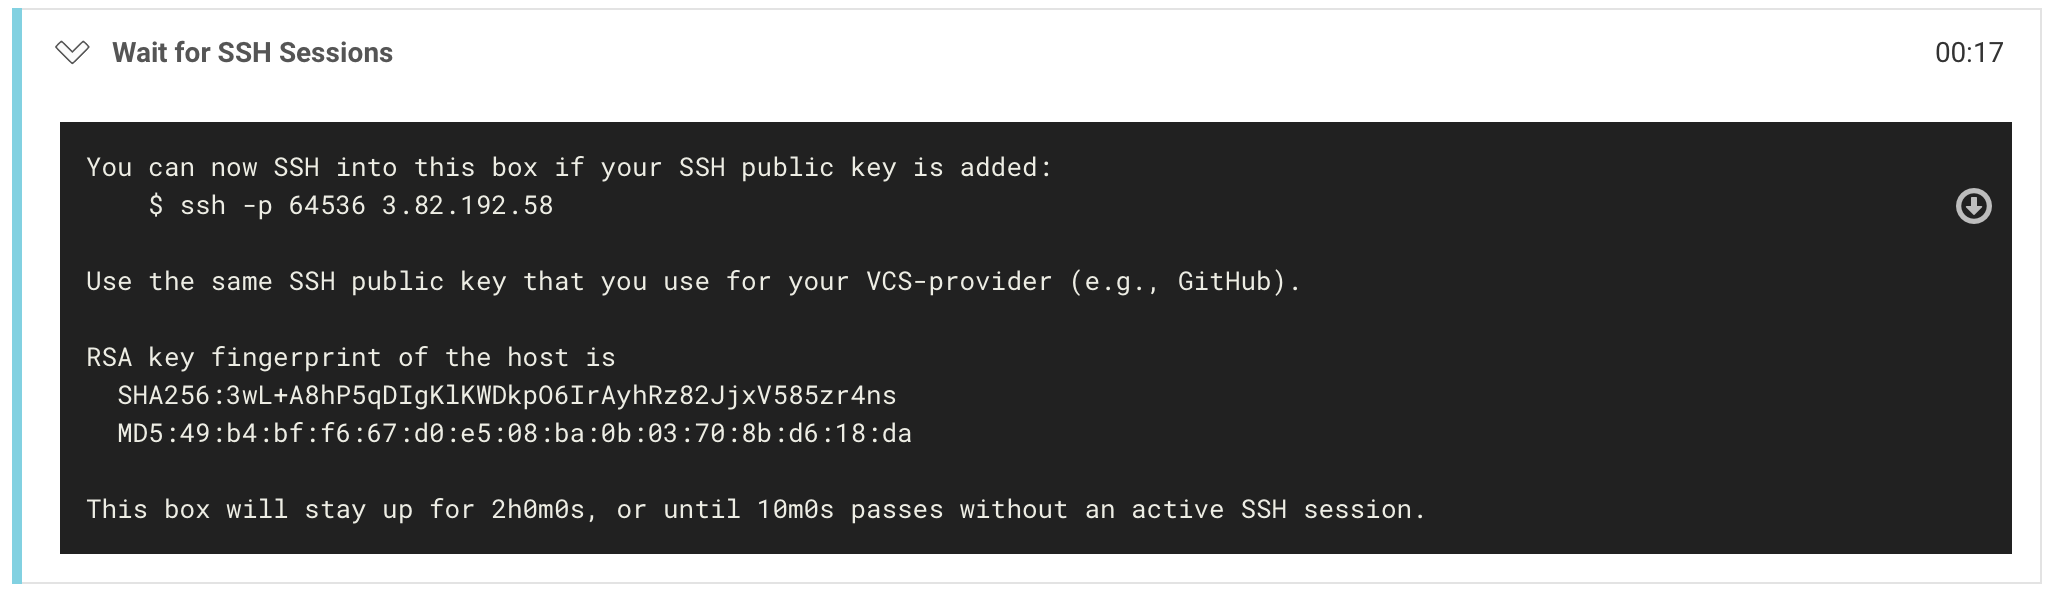
\includegraphics[width=1\linewidth]{../Images/SSH_Output}
  	\caption{Verbindungsdetails auf der Weboberfläche}
  	\label{fig:ssh-output}
\end{figure}

\begin{figure}[H]
	\centering
  	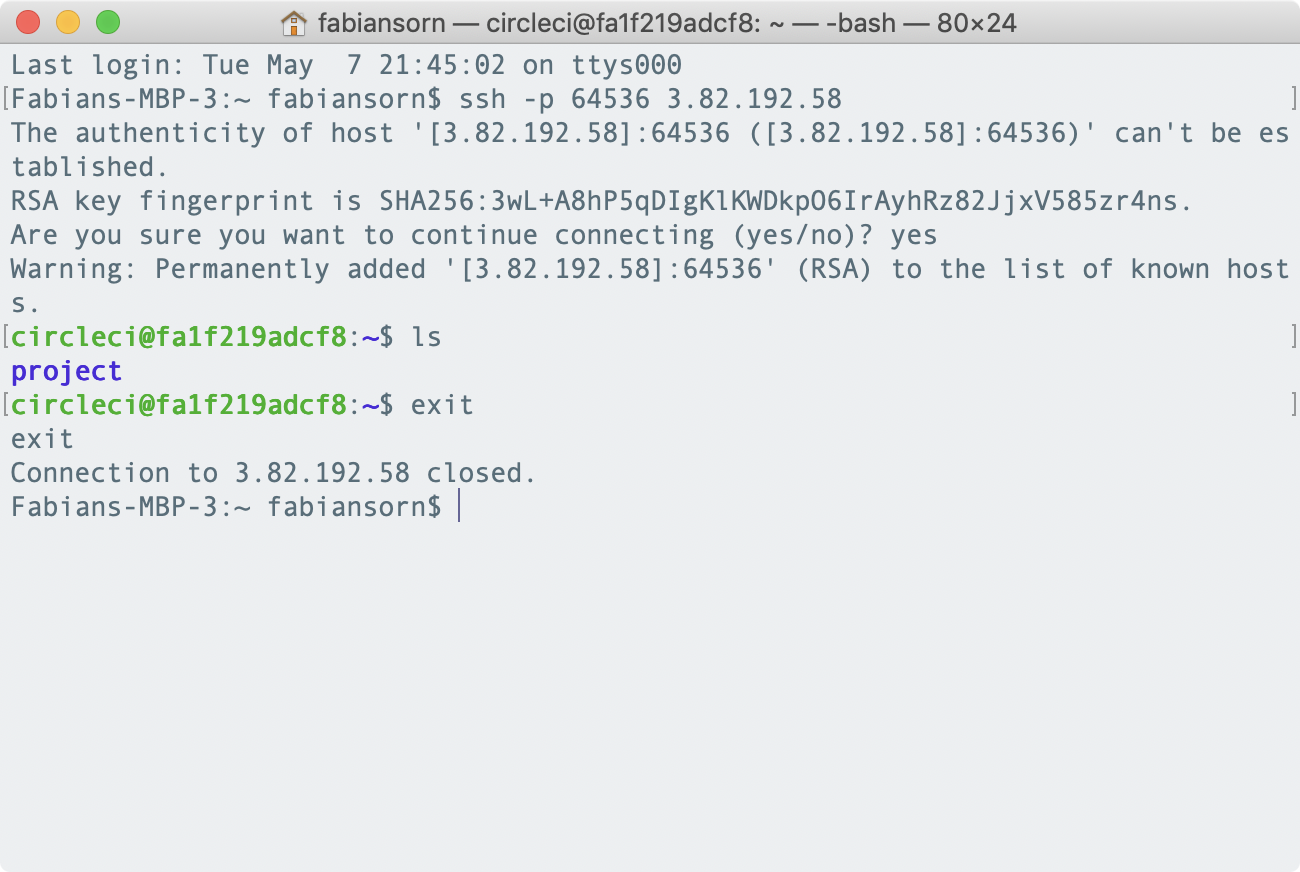
\includegraphics[width=0.7\linewidth]{../Images/Interact}
  	\caption{Aktive SSH Verbindung mit dem Circle CI Docker Container}
  	\label{fig:interact}
\end{figure}

\subsection{Verbesserungen der Performance}
Um Builds so effizient wie möglich auszuführen, unterstützt Circle CI sowohl eine nebenläufige Ausführung von Jobs, als auch Aufteilung und parallele Ausführung von Tests. Jobs, die nicht von einander abhängig sind, führt Circle CI bereits automatisch nebenläufig aus. Bei der Parallelisierung von Tests hingegen, muss vom Nutzer spezifiziert werden, wie die einzelnen Testdateien aufgeteilt werden sollen. Dabei gibt es folgende Möglichkeiten der Aufteilung:
\begin{enumerate}
	\item Automatische Verteilung mit Hilfe der CLI auf die zur Verfügung stehenden Container.
    \item Aufteilung basierend auf dem Namen der Testdateien
    \item Aufteilung basierend auf der Größe der Testdateien
    \item Aufteilung nach Testdauer, falls deren Speicherung vom Nutzer konfiguriert wurde
\end{enumerate}
Die Aufteilung der Tests werden von der CLI in Form einer Textdatei realisiert. Diese kann dann durch eine Umgebungsvariable referenziert werden und die Aufteilung der Tests bei der Ausführung bekannt machen.

\section{Schnittstellen}
Circle CI bietet verschiedene Möglichkeiten der Interaktion, mit denen Benutzer der Plattform verschiedene Aufgaben erledigen kann.

\subsection{Command Line Interface}
Circle CI bietet ein Command Line Interface an, das es erlaubt, bestimmte lokale Aufgaben im eigenen Projekt auszuführen und mit der Circle CI Plattform zu interagieren. Eine Funktionalität ist beispielsweise die Kombination mehrerer Konfigurationsdateien zu einer größeren zusammenhängenden Datei. Des Weiteren lässt sich die lokale Konfigurationsdatei mit der CLI einfach validieren. Circle CI CLI bietet Entwicklern auch die Möglichkeit, Jobs lokal auf dem eigenen Rechner auszuführen, wenn auch mit Einschränkungen. Ganze Workflows oder Jobs in einer Single-Use VM können lokal mit der CLI nicht angestoßen werden.

\begin{figure}[H]
	\centering
  	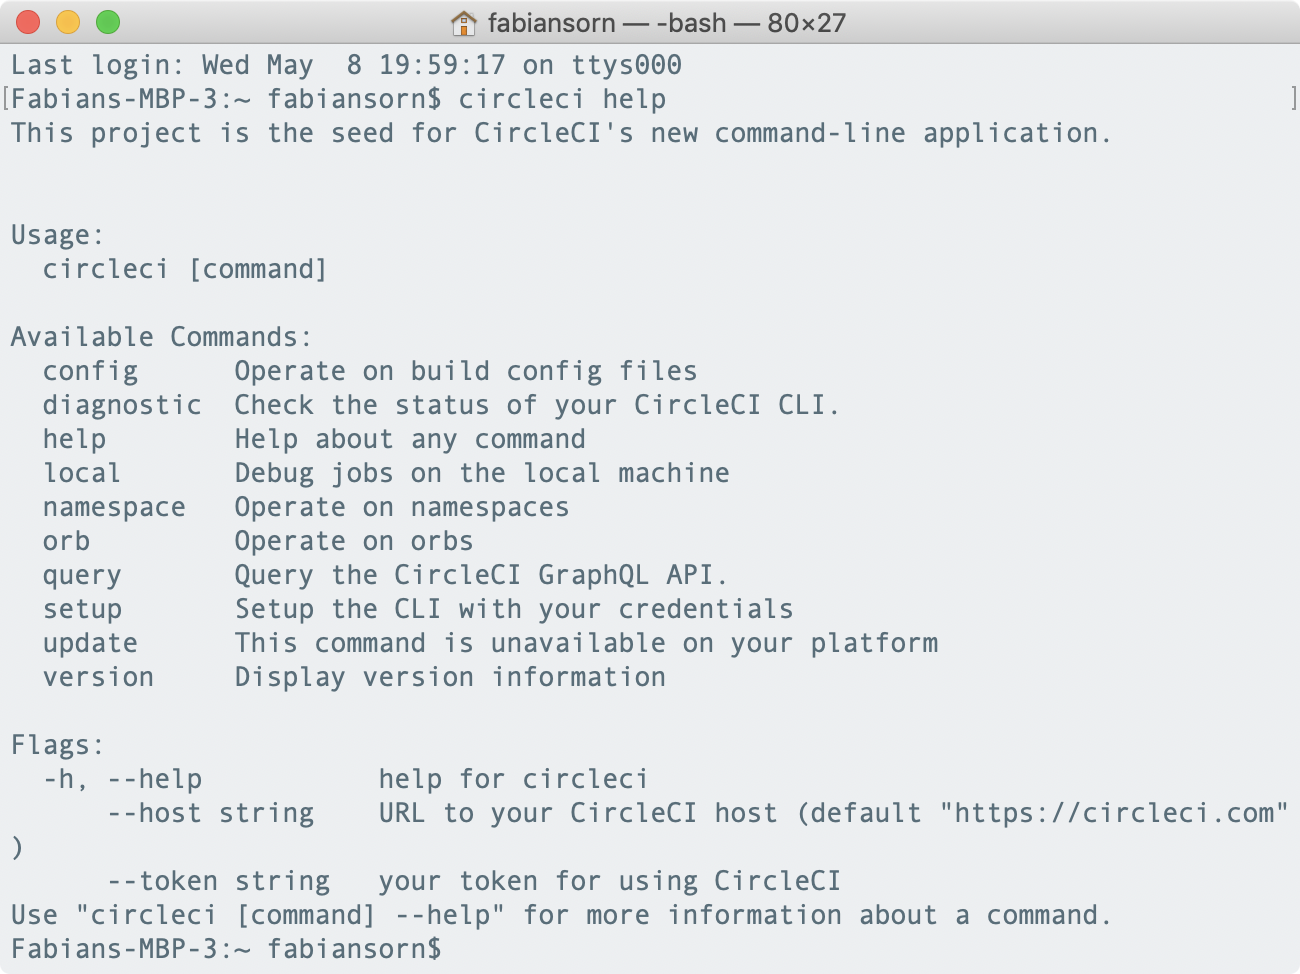
\includegraphics[width=0.7\linewidth]{../Images/CLI}
  	\caption{Command Line Interface}
  	\label{fig:cli}
\end{figure}

\subsection{Weboberfläche}
Die erste Anlaufstelle für Circle CI ist die Weboberfläche, die dem Nutzer viele Interaktions- und Überwachungsmöglichkeiten bietet. Wurden Änderungen in die Versionsverwaltung aufgenommen, so lässt sich über die Weboberfläche alle wichtigen Daten einsehen, die den angestoßenen Workflow betreffen, einsehen. Den in der Konfiguration definierten Workflow können wir hier grafisch einsehen sowie die Ergebnisse, Fehler, Artefakte und Zeiten der einzelnen Jobs. Die Logs der einzelnen Arbeitsschritte der Logs werden in der Weboberfläche dargestellt. Ist ein Job fehlgeschlagen, können dessen Logs hier eine gute erste Anlaufstelle für die Fehlersuche sein.

\begin{figure}[H]
	\centering
  	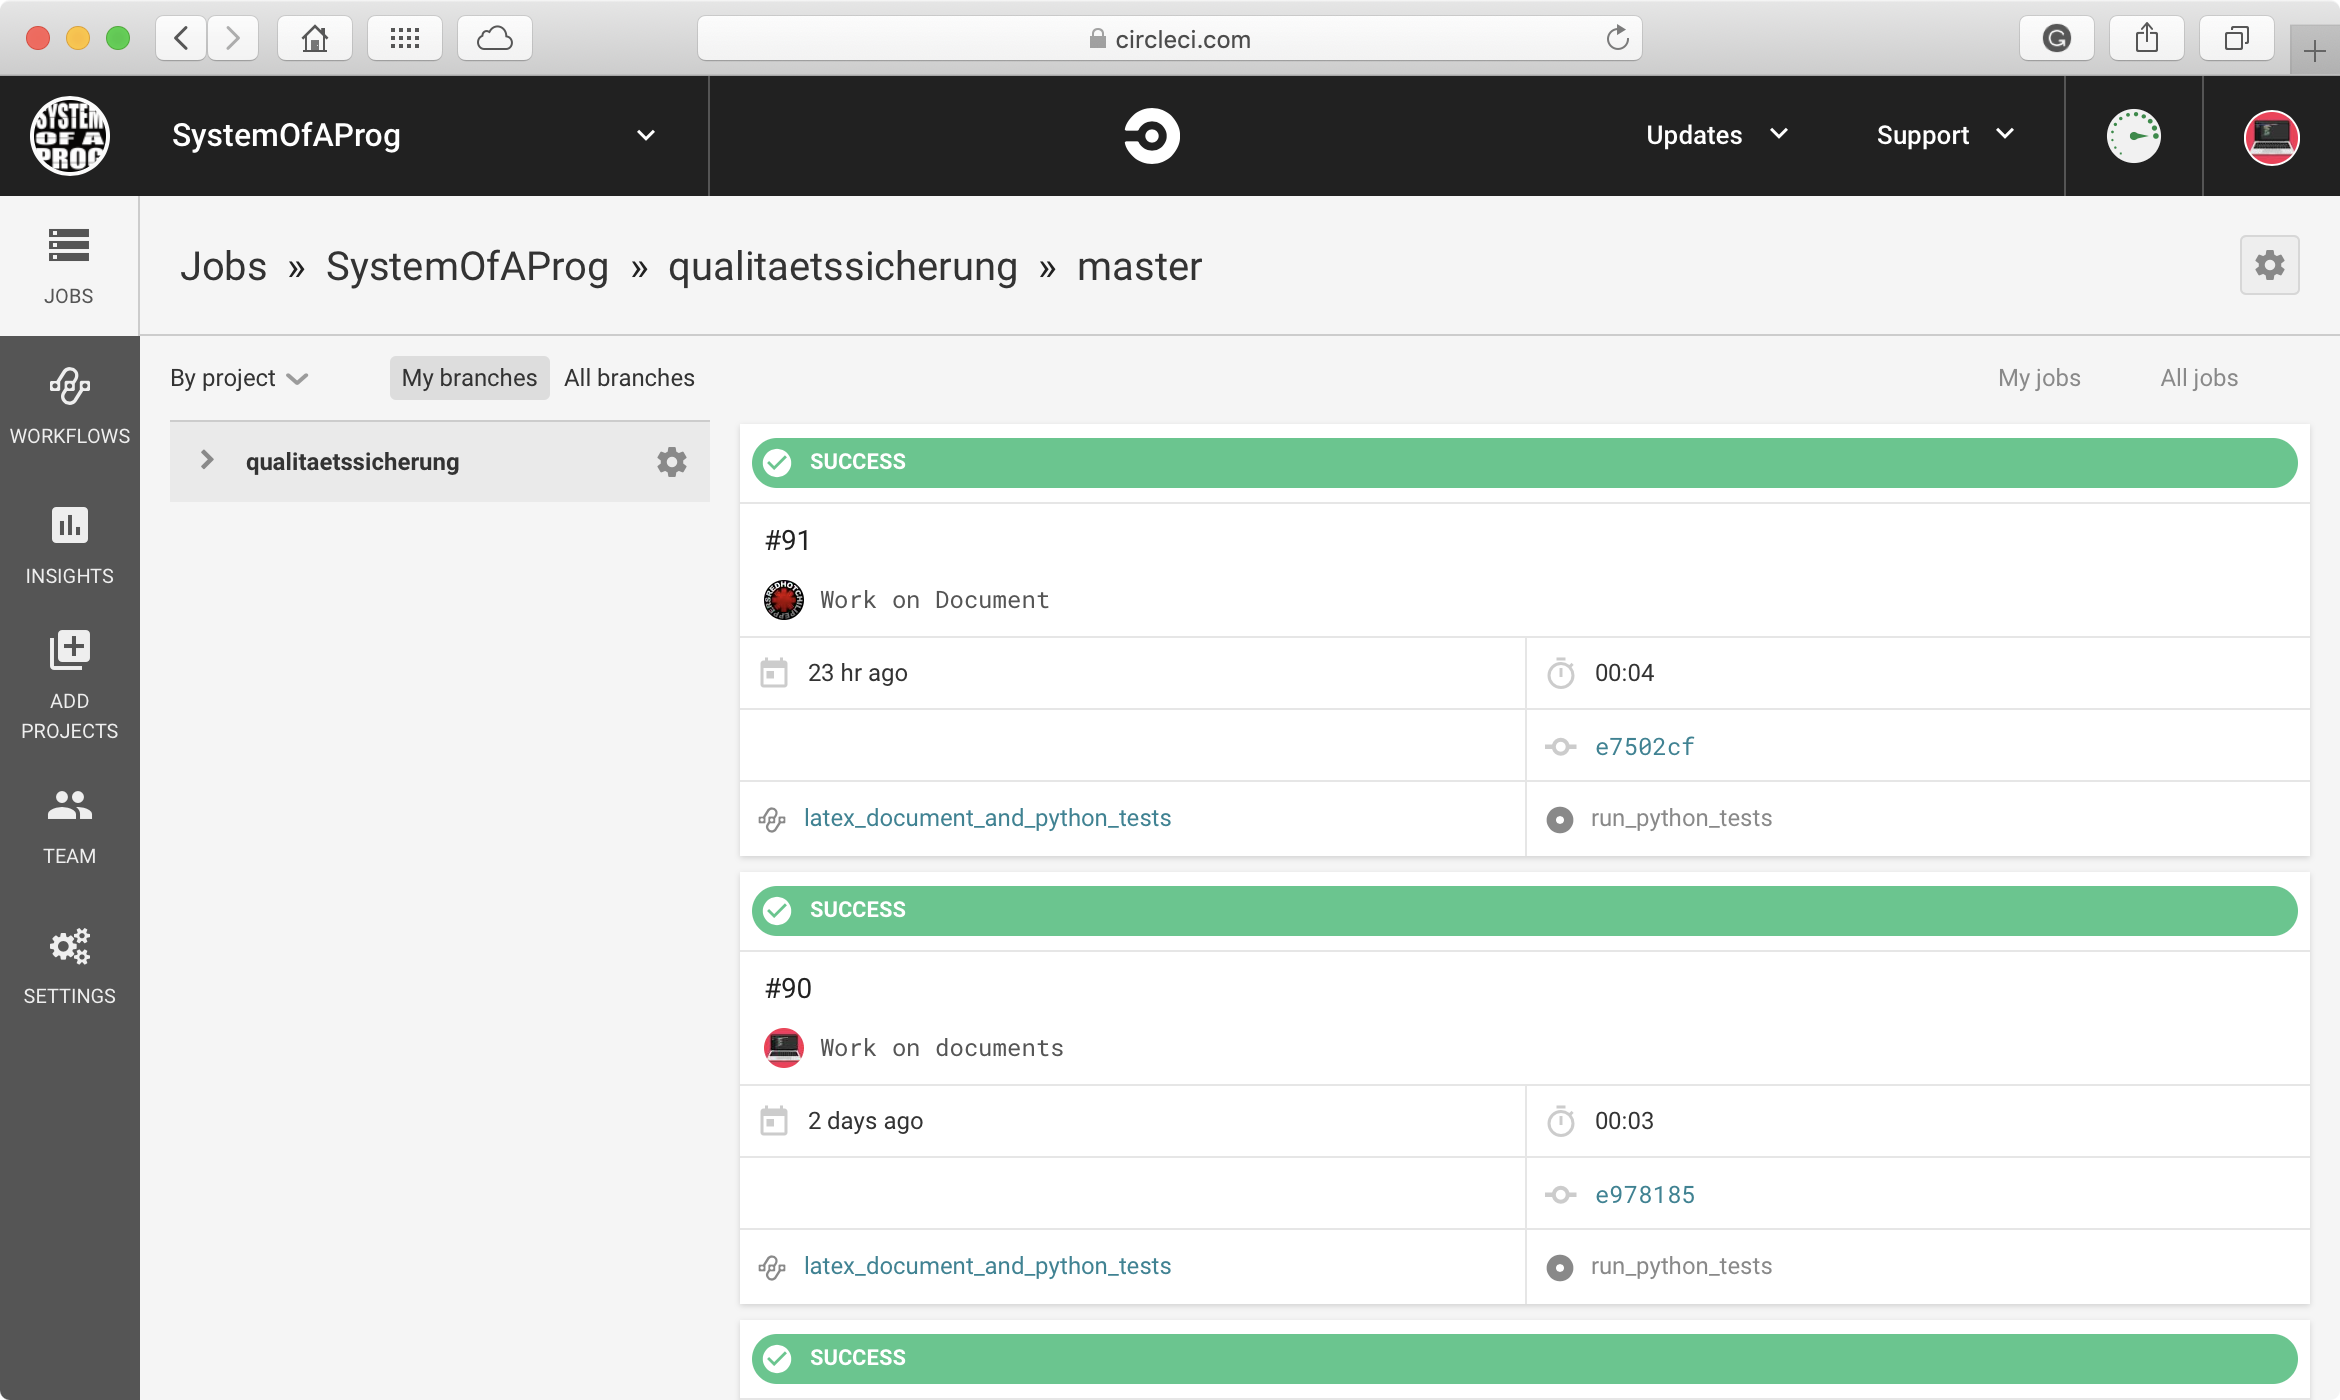
\includegraphics[width=1\linewidth]{../Images/Weboberflaeche}
  	\caption{Weboberfläche mit der Übersicht über die letzten Jobs}
  	\label{fig:weboberflaeche}
\end{figure}

\begin{figure}[H]
	\centering
  	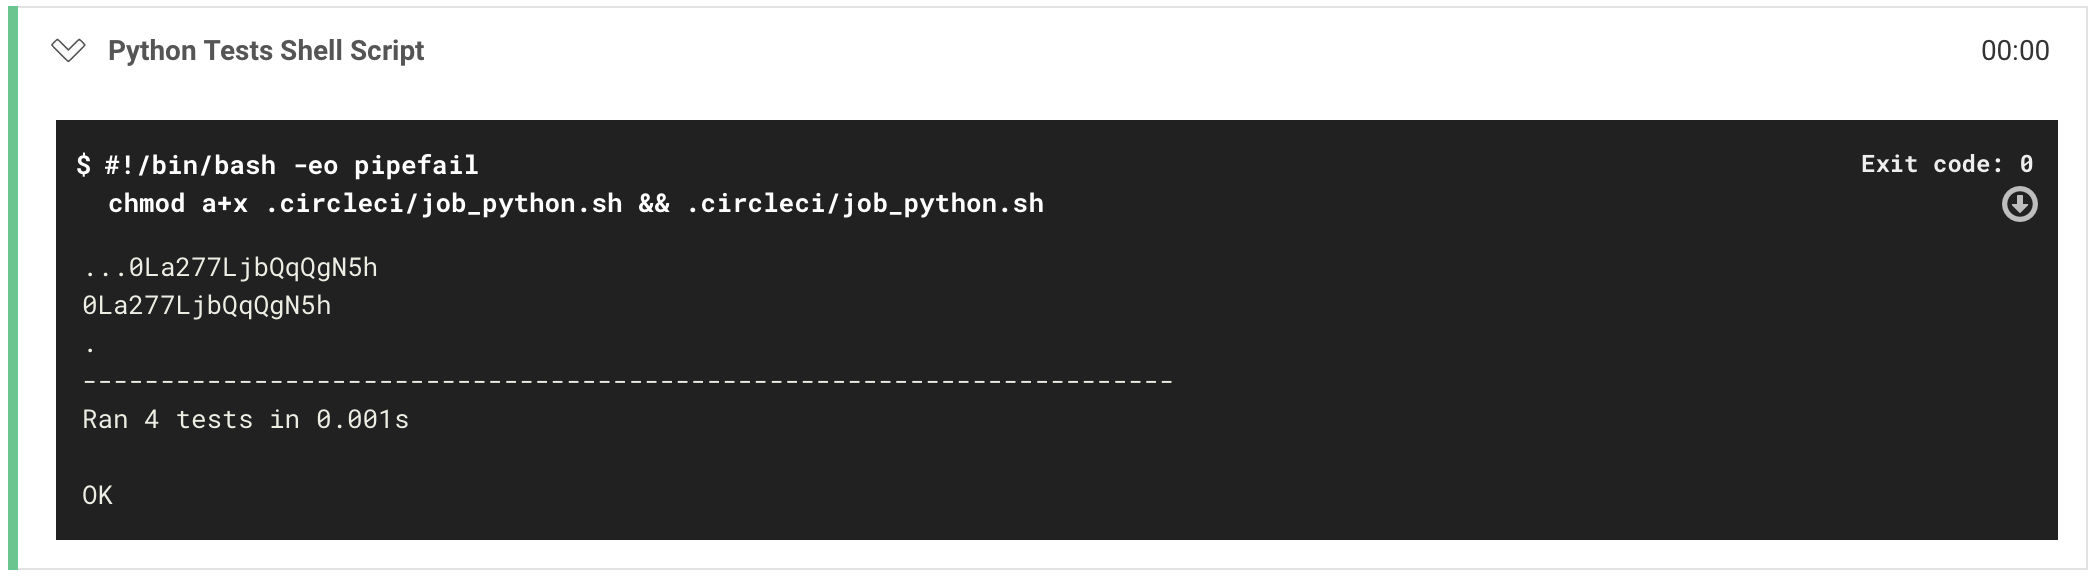
\includegraphics[width=1\linewidth]{../Images/Test_Logs}
  	\caption{Logs der Tests in der Weboberfläche}
  	\label{fig:testlogs}
\end{figure}

Neben dieser Funktionen können über die Weboberfläche auch neue Repositories in Circle CI aufgenommen werden oder bereits aufgenommene wieder entfernt werden, falls diese nicht mehr kontinuierlich integriert werden sollen.

\subsection{Circle CI API}
Eine letzte Interaktionsmöglichkeit mit Circle CI ist die Verwendung der über HTTP erreichbaren API. Diese kann beispielsweise über CLIs wie \textit{curl} verwendet werden, um die Ausführung bestimmter Jobs anzustoßen, Informationen über die eigenen Projekte abzurufen und viele mehr Funktionen. Neben der umfangreichen Weboberfläche eröffnet diese Schnittstelle neue Möglichkeiten, Informationen aus Circle CI so an anderen Stellen einzubinden, wie man dies möchte. Ein Beispiel hierfür wäre, Ergebnisse aus Circle CI Builds in einer anderen Webanwendung einzubinden.

\section {Vergleich zu anderen Tools und Anbieter}
\subsection {Vergleich zum Open Source Automatisierungsserver Jenkins}
Jenkins ist ein quelloffener Java basierter Automatisierungsserver, der sehr oft für kontinuierliche Integration und Auslieferung zum Einsatz kommt. Jenkins bietet selbst somit keine Software as a Service Lösung an, die private Anwender sofort nutzen können. Im Vergleich zu Circle CI bedeutet dies für den Nutzer allerdings gerade am Anfang einen erhöhten Aufwand für Administration und höhere Kosten, da eigene  Hardware bereitgestellt werden muss, auf der Jenkins installiert wird. Ein weiterer Unterschied zu Circle CI ist zudem, dass die Funktionalität von Jenkins stark von Plugins abhängig ist. Funktionalitäten wie das Auschecken von Git Repositories werden bei Jenkins durch Plugins realisiert. Auf der einen Seite erhöht dies die Flexibilität, auf der anderen Seite erhöht dies wiederum den administrativen Aufwand erhöht. Jenkins führt die zu automatisierenden Aufgaben in einem gewöhnlichen Verzeichnis im Dateisystem des Hosts aus. Dabei gibt es von Haus aus keine Abschottung des Testcodes zum Host Betriebssystem, auf dem die Jenkins Instanz läuft. Werden nun mehrere Aufgaben gleichzeitig über Multithreading realisiert, so sind dieses nicht von einander strikt getrennt und können sich gegenseitig beeinflussen. Möchte man die Tests in getrennten Bereichen ausführen, so muss dies vom Nutzer selbst umgesetzt werden. Wie bereits beschrieben setzt CircleCI im Gegensatz dazu von Haus aus auf von einander abgeschottete Container oder Virtuelle Maschinen. Eine parallelisierte Ausführung von Aufgaben, die gegenseitig strickt von einander getrennt sind, ist damit sehr einfach umzusetzen.

Abschließend kommt es auf den Umfang des Projekts und die Kapazität von Entwicklern und Administratoren an, welche Lösung besser geeignet ist. Sind die Projekte kleiner, gibt es wenig Kapazität für administrative Aufgaben und soll das Projekt so schnell wie möglich in kontinuierlich integriert werden, lohnt sich Circle CI oder eine andere Software as a Service Lösung. Wachsen die Projekte jedoch im Umfang und Entwicklungszeit, so lohnt sich der administrative Aufwand und das Anschaffen neuer Hardwarekapazitäten für Jenkins möglicherweise, da man hier gerade bei länger Entwicklungs-, Test- und Übersetzungsdauer auf lange Sicht die monatlichen Kosten von Circle CI einspart. Jenkins ist mit seinen vielen Plugins allerdings auch flexibler, während Erweiterungen bei Circle CI selbst entwickelt und integriert werden müssen.

\subsection {Vergleich zu SaaS CI Lösung Travis}
Travis CI ist im Gegensatz zu Jenkins genau wie Circle CI eine Cloud basierte CI Lösung. Die meisten der Vor- und Nachteile von Circle CI treffen somit auch auf Travis CI zu. Es existieren allerdings trotzdem einige kleinere Unterschiede zwischen den beiden CI Tools. Der erste Unterschied sind die Preise der beiden Tools. Travis CI ist lediglich für Open Source Projekte kostenlos verfügbar, während Circle CI auch für Geschäftskonten oder private Code Repositories bis zu bestimmten Grenzen kostenlos bleibt. Gerade für kleine Projekte mit geringer Build Zeit ist Circle CI daher besser geeignet, wenn der Code nicht öffentlich zugänglich ist. Für Open Source Projekte hingegen bietet Travis CI jedoch mehr Freiheiten. Im Gegensatz zu Circle CI unterstützt Travis CI Builds und Tests in einer Windows Umgebung. Circle CI plant diese allerdings nachzuliefern. Circle CI bietet dafür wiederum eine geringere Queueing Zeit für Builds, sowie bessere Kontrolle über Hardware Ressourcen. Ein weiterer Vorteil von Circle CI ist, die breitere Skalierbarkeit für größere Software Projekte. Dabei werden die Pakete mit wachsender Leistung allerdings auch stark im Preis. Travis CI bietet auf der anderen Seite einen breiter gefächerten Support für mehr Sprachen, sowie Build Matrizen, die es erlauben, Tests in verschiedenen Sprach- und Umgebungsversionen auszuführen.

Eine einfache Wahl zwischen den beiden Plattformen ist hier nur unter Berücksichtigung vieler Details
machbar. Eine einfache Empfehlung ist aufgrund ihrer Ähnlichkeit nur schwer zu geben.

\section{Beispielprojekte}
Nach den grundlegenden Konzepten von Circle CI bietet es sich besonders an, ein eigenes kleines
Beispielprojekt in Circle CI zu integrieren. Hierbei gehen wir in den nächsten zwei Unterabschnitte
auf zwei sehr überschaubare Beispiele ein.

\subsection{Python Projekt}
Das erste kleine Projekt ist ein in Python geschriebener Quelltext, dass auf Basis eines Master-Passwortes, eines Nutzernamen und eines Dienstes ein Passwort generieren soll, das einfach mit Hilfe des Master Passwortes wiederherstellbar ist. Der Nutzer müsste sich so nur ein einziges Passwort merken und könnte für verschiedene Dienste spezifische Passwörter generieren. Die Generierung eines solchen Passwortes lässt sich sehr gut mit einfachen Unit Tests überprüfen. Die Implementierung ist hierbei zweitrangig und stellt keinerlei Ansprüche an die Sicherheit dieser generierten Passwörter, da die Implementierung lediglich zu Demonstrationszwecken dient. Im Anhang befindet sich ein Auszug der wichtigsten Dateien, die Teil des Projekts sind.

Zusätzlich legen wir eine zweite Klasse \textit{PasswordManagerUser} an, die auf unserem \textit{Passwordmanager} aufbaut. Auch hier legen wir einen weiteren Test an, der die Funktionalität der Klasse prüfen soll. Fügen wir nun Änderungen in der PasswortManager Klasse hinzu, so müssen wir in diesem Fall darauf achten, dass wir dabei auch Klassen anpassen, die vom PasswordManager abhängig sind. Eine Gefahr wäre nun, dass genau die nicht gemacht wird und der Fehler unentdeckt bleibt, wenn wir nach den Änderungen des PasswordManager lediglich lokal dessen Tests ausführen. Da wir allerdings nicht immer wissen welche Klassen und Methoden inhaltlich zusammenhängen, ist es auch  schwer, alle "betroffenen" Tests auszuführen, womit uns lediglich übrig bleibt, alle Tests auszuführen die es im Projekt gibt, wenn wir sicher sein wollen, dass unsere Änderungen keinen negativen Einfluss auf andere Code Stellen hat. Das Problem ist allerdings, dass die Ausführung der Tests gerade bei sehr großen Projekten oft Minuten oder Stunden dauern kann. Der Rechner des Entwicklers wäre in dieser Zeit blockiert oder nur eingeschränkt nutzbar. Circle CI erlaubt es in diesem Fall, die Tests automatisch mit dem gepushten Commit auszuführen. Der Entwickler kann lokal uneingeschränkt weiterarbeiten und wird über auftretende Fehler benachrichtigt und kann diese im Anschluss reparieren.

Bei einem Blick auf den Code fällt auf, dass dieser keinerlei Circle CI spezifischen Elemente wie Abhängigkeiten beinhaltet. Wie in der Anleitung bereits erwähnt, diese auch nicht, sondern lediglich eine Anleitung, was Circle CI mit dem Projekt tun soll. Hierfür legen wir in unserem Projekt einen Ordner
\textit{.circleci} mit einer Datei \textit{config.yml} an. In der ausführlichen Dokumentation von Circle CI
findet sich eine Vielzahl von Feldern, die den Ablauf der Tests beeinflussen. Auf den genauen Inhalt der Konfigurationsdatei gehen wir etwas später genauer ein.

\subsection{Latex Dokumenten Generation}

Nach der erfolgreichen Integration des Python Projektes stellte sich die Frage, welche Aufgaben Circle CI noch übernehmen kann, die vielleicht nicht in der offiziellen Dokumentation erwähnt werden. Daher entschieden wir uns zu versuchen, das Bauen dieses in Latex verfassten Dokuments als Job in Circle CI zu integrieren, obwohl keinerlei Unterstützung für das Übersetzen von Latex Dateien geboten wird. Für die Übersetzung benötigen wir lediglich eine Umgebung, in der eine passende Latex Distribution bereitgestellt ist, die das Dokument beispielsweise mit einem einfachen \textit{pdflatex} Befehl übersetzt werden kann. Circle CI bietet allerdings keine virtuelle Maschine oder Docker Container, die für diese Aufgabe geeignet war. Daher entschieden wir uns für die Einbindung des Docker Containers \textit{koppor/texlive}, der nicht von Circle CI selbst stammt, aber mit der Plattform problemlos funktionieren soll. In der offiziellen Dokumentation von Circle CI finden sich weitere Hinweise auf die Erstellung eigener Docker basierten Umgebungen. Im Gegensatz zum Python Projekte entsteht hier auch, ähnlich wie bei Projekten in Programmiersprachen, die gebaut werden, ein Endprodukt. Der Job für den Bau des Dokumentes wurde dabei so konfiguriert, dass 

\subsection{Konfiguration des Circle CI Workflows}
In diesem Abschnitt möchten wir etwas genauer auf den Inhalt der Konfigurationsdatei unseres Projektes eingehen, deren Inhalt sich im Anhang befindet. Die Datei beginnt mit der Angabe der Version von Circle CI, die verwendet werden soll. Wir entscheiden uns für die Aktuellste Version 2.1.

\begin{figure}[H]
	\centering
  	
\includegraphics[width=1\linewidth]{../Images/Config/Version}
  	\caption{Definition der in Circle CI zu verwendenden Version}
  	\label{fig:version}
\end{figure}

Das nächste Feld listet die Jobs auf, die Circle CI ausführen sollen. Beide werden später bei der Angabe der Reihenfolge bei der Ausführung über ihre Namen referenziert. Die Definition eines Jobs besteht mindestens aus zwei Teilen: der Angabe der Umgebung, in der der Job ausgeführt werden soll und die einzelnen Schritte in Form von Shell Befehlen. In beiden Fällen entscheiden wir uns für die Verwendung eines Docker Containers, der alle wichtigen Abhängigkeiten wie eine Python Installation oder eine Latex Distribution für das Übersetzen unseres Dokument mitbringt. Alternativ könnten wir hier auch Virtuelle Maschinen auf Linux oder macOS Basis verwenden, wenn wir diese für unseren Job benötigen würden.
Darauf folgt die Liste der Shell Befehle, die Circle CI sequentiell anstößt. In beiden Jobs beginnen wir mit dem auschecken des Projektes aus der Versionsverwaltung, was mit dem Keyword \textit{checkout} anstoßen wird. Im Anschluss folgen die nächsten Arbeitsschritte, die durch das Keyword run gekennzeichnet werden. Im Fall unserer Projekte haben wir alle Befehle in ein separates Shell Script extrahiert.

\begin{figure}[H]
	\centering
  	
\includegraphics[width=1\linewidth]{../Images/Config/Python}
  	\caption{Shell Script mit den Befehlen zum Ausführen der Python Tests}
  	\label{fig:python}
\end{figure}

\begin{figure}[H]
	\centering
  	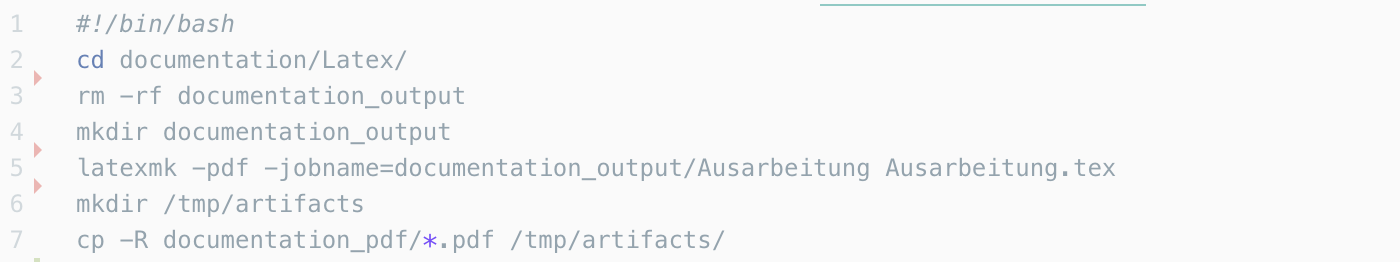
\includegraphics[width=1\linewidth]{../Images/Config/Latex}
  	\caption{Shell Script mit den Befehl zum Bauen und Speichern des Latex Dokuments}
  	\label{fig:latex}
\end{figure}

In der Konfigurationsdatei wird dieses Script dann aufgerufen. Alternativ könnten die einzelnen Befehle auch direkt in der Konfigurationsdatei in Form einzelner Steps definiert und benannt werden. Diese Variante ist zwar etwas aufwändiger zu schreiben, führt aber später bei der Auswertung zu einer klareren Trennung der einzelnen Arbeitsschritte.
Eine Besonderheit im Latex Job ist das Speichern von Build Artefakten, um diese später über die Weboberfläche abzurufen. Im Fall unseres Dokuments bietet es sich besonders an, dieses bei erfolgreichem Setzen als Artefakt zu speichern. Dafür definieren wir lediglich welche Dateien oder Ordner später abrufbar sein sollen. Im Shell Script für den Latex Job haben wir das Dokument bereits in einen separaten Ordner \textit{/tmp/artifacts/} gespeichert. Diesen können wir nun in unserer Konfiguration angeben. Wurde der Build erfolgreich ausgeführt, kann die PDF des jeweiligen Builds nun über die Weboberflächen von Circle CI abgerufen und heruntergeladen werden.

\begin{figure}[H]
	\centering
  	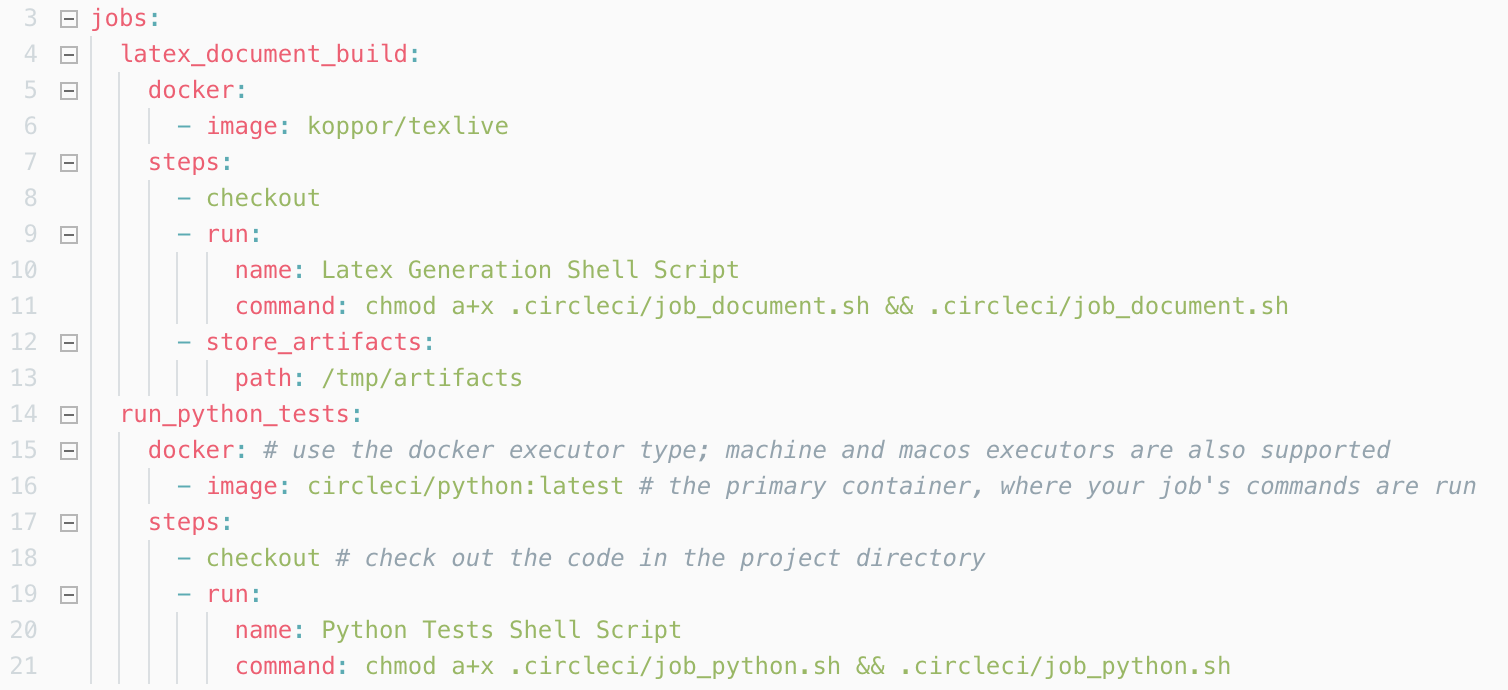
\includegraphics[width=1\linewidth]{../Images/Config/Jobs}
  	\caption{Definition der Jobs latex\_document\_build und run\_python\_tests}
  	\label{fig:jobs}
\end{figure}

Nachdem wir unsere beiden Jobs definiert haben, definieren wir den Workflow in dem die Reihenfolge festgelegt wird, in der die einzelnen Jobs ausgeführt werden. In unserem Fall sind beide Jobs unabhängig von einander und müssen nicht in einer bestimmten Reihenfolge sequentiell ausgeführt werden. Daher verweisen wir unter jobs auf beide Jobs ohne weitere Angaben. Die beiden Jobs werden somit parallel unabhängig von einander ausgeführt. Wären sie abhängig von einander, könnten wir über ein zusätzliches Feld require in der Definition des Workflows auf einen anderen Job verweisen, der beendet sein muss, bevor der aktuelle Job anfängt. So kann beispielsweise der Deployment Job auf die Ergebnisse des Build Jobs warten.

\begin{figure}[H]
	\centering
  	
\includegraphics[width=1\linewidth]{../Images/Config/Workflow}
  	\caption{Definition des Workflows basierend auf den einzelnen Jobs}
  	\label{fig:workflow}
\end{figure}

\section{Abschließende Zusammenfassung}
Circle CI bietet für eine breit gefächerte Nutzerbasis eine gute Möglichkeit, die Qualität ihrer Software durch kontinuierliches Ausführen von Builds und Tests zu erhöhen. Gerade für kleinere Projekte bieten sich Plattformen wie Circle CI besonders an, da sie bei geringer Ausführungszeit oft kostenlos sind, der Aufwand für das initiale Einbinden des Projektes sehr gering ist und die Dokumentation der einzelnen Features sehr ausführlich ist. Neben Circle CI gibt es allerdings auch viele weitere Anbieter von CI Lösungen, die fast identische Vor- und Nachteile mit sich bringen. Unterschiede sind hier oft besonders im Detail zu finden. Welche Plattform sich in jedem einzelnen Fall am besten eignet, muss im speziellen Fall untersucht werden.
Bei größeren Projekten bietet sich Circle CI besonders durch die 

\end{document}